%############################################################################################
%###################### 									    												 ######################
%######################  Aten��o este n�o � o documento atualizado!!!  ######################
%######################									     													 ######################
%############################################################################################

\documentclass[journal,harvard,american,english]{sbatex}
\usepackage{amssymb,amsmath,babel,graphicx,float,array,ae}
\usepackage[latin1]{inputenc}
\sloppy
\hyphenpenalty=10000 % Para n�o hifenizar

\citationmode{abbr}
\citationstyle{dcu}
%\bibliographystyle{dcu}

\newcommand\real{\mathbb{R}}
\newcommand{\req}[1]{(\ref{#1})}

\edicaosbai{VII}          % em numerais romanos letras maiusculas
\messbai{setembro}       % mes em que trasncorrera o simposio, minusculas
\anosbai{2005}           % ano no format AAAA
\localsbai{S�o Lu�s}        % Cidade onde ocorrera o simposio, primeira letra
 
\begin{document}

\title{Mobile Robot Trajectory Tracking Using Model Predictive Control}

\author{Felipe K�hne}{kuhne@eletro.ufrgs.br}
\address{Universidade Federal do Rio Grande do Sul\\Departamento de Engenharia El�trica\\Av. Oswaldo Aranha, 103 -- CEP 90035-190\\Porto Alegre, RS, Brasil}

\author[1]{Jo�o Manoel Gomes da Silva Jr.}{jmgomes@eletro.ufrgs.br}
\author[1]{Walter Fetter Lages}{fetter@eletro.ufrgs.br}

\maketitle

\begin{abstract}
This work focus on the application of model-based predictive control (MPC) to the trajectory tracking problem of nonholonomic wheeled mobile robots (WMR). The main motivation of the use of MPC in this case relies on its ability in considering, in a straightforward way, control and state constraints that naturally arise in practical problems. Furthermore, MPC techniques consider an explicit performance criterion to be minimized during the computation of the control law. The trajectory tracking problem is solved using two approaches: (1) nonlinear MPC and (2) linear MPC. Simulation results are provided in order to show the effectiveness of both schemes. Considerations regarding the computational effort of the MPC are developed with the purpose of analysing the real-time implementation viability of the proposed techniques.
\end{abstract}
\keywords{Mobile robots, trajectory tracking, nonholonomic systems, model-based predictive control.}

%%%%%%%%%%%%%%%%%%%%%%%%%%%%%%%%%%%%%%%
\section{Introduction}\label{sec:intro}
The field of mobile robot control has been the focus of active research in the past decades. Despite the apparent simplicity of the kinematic model of a wheeled mobile robot (WMR), the design of stabilizing control laws for those systems can be considered a challenge due to the existence of nonholonomic (non-integrable) constraints. Due to Brockett's conditions~\cite{brockett82}, a smooth, time-invariant, static state feedback control law cannot be used to stabilize a nonholonomic system at a given configuration. To overcome this limitation most works use non-smooth and time-varying control laws~\cite{bloch89,samson91,canudas92,yamamoto94,murray97}. On the other hand, this limitation can be avoided when the objective is the tracking of a pre-computed trajectory~\cite{kanayama90,pomet92,yang99,do02,sun05}.

Traditional techniques for the control of nonholonomic WMRs often do not present good results, due to constraints on inputs or states that naturally arise. Also, in general, the resulting closed-loop trajectory presents undesirable oscillatory motions. Furthermore, tuning parameters are difficult to choose in order to achieve good performance since the control laws are not intuitively obtained. Model-based predictive control (MPC) appears therefore as an interesting and promising approach for overcoming the problems above mentioned. In particular, by using MPC it follows that: the tuning parameters are directly related to a cost function which is minimized in order to obtain an optimal control sequence; constraints on state and control inputs can be considered in a straightforward way. Thus, control actions that respect actuators limits are automatically generated. By considering state constraints, the configuration of the robot can be restricted to belong to a safe region~\cite{kuhne05}. On the other hand, the main drawback of MPC schemes is related to its computational burden which, in the past years, had limited its applications only to sufficient slow dynamic systems. However, with the development of increasingly faster processors and efficient numerical algorithms, the use of MPC in faster applications, which is the case of WMRs, becomes possible. 

Although MPC is not a new control method, works dealing with MPC of WMRs are sparse. In~\cite{ollero91,rico99}, GPC (Generalized Predictive Control) is used to solve the path following problem. In that work, it is supposed that the control acts only in the angular velocity, while the inear velocity is constant. Hence, an input-output linear model is used to compute the distance between the robot and a reference path. Note that differently from the trajectory tracking problem, in the path following the reference is not time-parametrized. In~\cite{ortega96} a nonlinear model of the WMR is used for trajectory tracking. The problem is solved considering unknown obstacles in the configuration space. A neural network helps to solve the optimization problem. Also, in~\cite{yang98} the path following problem is solved by using a neural network to predict the future behavior of a car-like WMR. The modeling errors are corrected on-line with the neural network model. Using a nonlinear model of the robot, in~\cite{essen01} a nonlinear MPC (NMPC) algorithm in state-space representation is developed, which is applied to both problems of point stabilization and trajectory tracking. A modified cost function to be minimized is proposed. Accordingly to the authors, the MPC developed in that work can not be applied in real-time, given the high computational effort necessary in the optimization problem.

In this paper, we are interested in the application of MPC schemes to control a WMR in the problem of trajectory tracking. Two approaches based on state-space representation of the kinematic model of a nonholonomic WMR are developed. First, a nonlinear MPC (NMPC) is developed, which leads to a non-convex optimization problem. In a second approach a linear technique is proposed to overcome the problem related to the computational burden of the NMPC. The fundamental idea consists in using a successive linearization approach, as briefly outlined in~\cite{henson98}, yielding a linear, time-varying description of the system. From this linear description, the optimization problem to be solved at each sampling period is a quadratic program (QP) one, which is convex and computationally less expressive than the optimization problem that arises in the classical NMPC.

Finally, analysis regarding the computational effort are carried out in order to evaluate the real-time implementability of the MPC strategies proposed here.


%%%%%%%%%%%%%%%%%%%%%%%%%%%%%%%%%%%%%%%%%%%%%%
\section{Problem Formulation}\label{sec:model}
A mobile robot made up of a rigid body and non deforming wheels is considered (Fig.~\ref{fig:robot}). It is assumed that the vehicle moves without slipping on a plane, i.e., there is a pure rolling contact between the wheels and the ground. The kinematic model of the WMR is then given by~\cite{campion96}:
\begin{equation}
\label{eqn:model}
	\left\{
		\begin{aligned}
			\dot x	  &= v\cos\theta \\
			\dot y	  &= v\sin\theta \\
			\dot \theta &= w
		\end{aligned}
	\right.
\end{equation}
or, in a more compact form as
\begin{equation}\label{eqn:modelshort}
	\dot{\bf x} = f({\bf x},{\bf u}),	
\end{equation}
\noindent where ${\bf x}=[x~~y~~\theta]^T$ describes the configuration (position and orientation) of the center of the axis of the wheels, $C$, with respect to a global inertial frame $\{O,X,Y\}$. ${\bf u}=[v~~w]^T$ is the control input, where $v$ and $w$ are the linear and the angular velocities, respectively.
\begin{figure}
	\centering
	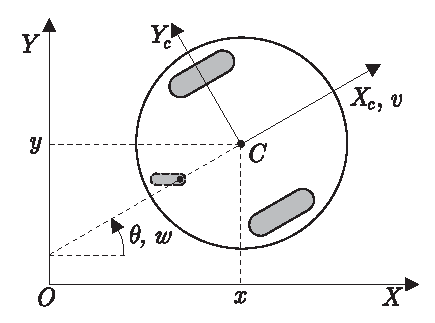
\includegraphics[width=0.68\linewidth]{Figuras/robot.eps}
	\caption{Coordinate system of the WMR.}
	\label{fig:robot}
\end{figure}

As described in the next sections, in MPC a prediction model is used and the control law is computed in discrete-time. Thus, a discrete-time representation of this model becomes necessary. Considering a sampling period $T$, a sampling instant $k$ and applying the Euler's approximation to~\req{eqn:model}, we obtain the following discrete-time model for the robot motion:
\begin{equation*}\label{eqn:discretemodel}
	\left\{
		\begin{aligned}
			x(k+1)	    &= x(k) + v(k)\cos\theta(k)T \\
			y(k+1)	    &= y(k) + v(k)\sin\theta(k)T \\
			\theta(k+1) &= \theta(k) + w(k)T \\
		\end{aligned}
	\right.
\end{equation*}
or, in a compact representation,
\begin{equation}\label{eqn:discretemodelshort}
	{\bf x}(k+1) = f_d({\bf x}(k),{\bf u}(k))
\end{equation}

The problem of trajectory tracking can be stated as to find a control law such that
\begin{equation*}
	{\bf x}(k)-{\bf x}_r(k)=0
\end{equation*}
where ${\bf x}_r$ is a known, pre-specified reference trajectory. It is usual in this case to associate to this reference trajectory a {\em virtual} reference robot, which has the same model than the robot to be controlled. Thus, we have:
\begin{equation}\label{eqn:refmodel}
	\dot{\bf x}_r = f({\bf x}_r,{\bf u}_r),
\end{equation}
or, in discrete-time, ${\bf x}_r(k+1) = f_d({\bf x}_r(k),{\bf u}_r(k))$.


%%%%%%%%%%%%%%%%%%%%%%%%%%%%%%%%%%%%%%%%%%%%%%%%%%%%
\section{The Nonlinear MPC Approach}\label{sec:nmpc}
In this section, the trajectory tracking problem is solved with a NMPC strategy. In order to evaluate the performance of the approach, simulation results are shown. 

MPC is an optimal control strategy that uses the model of the system to obtain an optimal control sequence by minimizing an objective function. At each sampling instant, the model is used to predict the behavior of the system over a prediction horizon. Based on these predictions, the objective function is minimized with respect to the future sequence of inputs, thus requiring the solution of a constrained optimization problem for each sampling instant. Although prediction and optimization are performed over a future horizon, only the values of the inputs for the current sampling interval are used. The same procedure is repeated at the next sampling instant with updated process measurements and a shifted horizon. This mechanism is known as {\it moving} or {\it receding horizon} strategy, in reference to the way in which the time window shifts forward from one sampling instant to the next one~\cite{camacho99,allgower99}.

From~\req{eqn:discretemodelshort}, the prediction of the robot motion is obtained as follows:
\begin{equation*}
	{\bf x}(k+j+1|k)=f_d({\bf x}(k+j|k),{\bf u}(k+j|k)),
\end{equation*}
where $j\in[0,N-1]$ and the notation $a(m|n)$ indicates the value of $a$ at the instant $m$ predicted at instant $n$. By defining error vectors $\tilde{\bf x}={\bf x}-{\bf x}_r$ and $\tilde{\bf u}={\bf u}-{\bf u}_r$, we can formulate the following objective function to be minimized:
\begin{multline}\label{eqn:cost}
	\Phi(k) = \sum_{j=1}^{N}\tilde{\bf x}^T(k+j|k){\bf Q}\tilde{\bf x}(k+j|k) + \\ + \tilde{\bf u}^T(k+j-1|k)\tilde{\bf R}{\bf u}(k+j-1|k),
\end{multline}
where $N$ is the prediction horizon and ${\bf Q}\geq 0$, ${\bf R}>0$ are weighting matrices for error in the state and control variables, respectively.

We consider also the existence of bounds in the amplitude of the control variables:
\begin{equation}\label{eqn:restu}
	{\bf u}_{min} \leq {\bf u}(k+j|k) \leq {\bf u}_{max},
\end{equation}
where ${\bf u}_{min}$ stands for the lower bound and ${\bf u}_{max}$ stands for the upper bound\footnote{The symbol $\leq$ stands for componentwise inequalities in this case.}. Note that we can write~\req{eqn:restu} in a more general form as 
\begin{equation*}
	{\bf Du}(k+j|k)\leq{\bf d}
\end{equation*}
with:
\begin{equation*}\label{eqn:const2}
	{\bf D} = \begin{bmatrix} {\bf I} \\ -{\bf I} \end{bmatrix}, \qquad 
	{\bf d} = \begin{bmatrix} {\bf u}_{max} \\ -{\bf u}_{min} \end{bmatrix},
\end{equation*}
and, in a similar way, state constraints can be generically expressed by ${\bf Cx}(k+j|k)\leq{\bf c}$.

Hence, the nonlinear optimization problem can be stated as:
\begin{equation}\label{eqn:optim}
	{\bf x}^\star,{\bf u}^\star = \arg\min_{{\bf x},{\bf u}}\left\{\Phi(k)\right\}
\end{equation}
s. a.
\begin{align}
	{\bf x}(k|k)     &= {\bf x}_0, \label{eqn:restci} \\
	{\bf x}(k+j+1|k) &= f_d({\bf x}(k+j|k),{\bf u}(k+j|k)), \label{eqn:restmodel} \\
	{\bf Du}(k+j|k)  &\leq {\bf d}, \label{eqn:restgu}
\end{align}
where $j\in[0,N-1]$. ${\bf x}_0$ is the initial condition which corresponds to the value of the states measured at the current instant. Constraint~\req{eqn:restmodel} represents the prediction model and~\req{eqn:restgu} is the control constraint which may be present or not in the optimization problem. Notice that the decision variables are both state and control variables.

The optimization problem~\req{eqn:optim}--\req{eqn:restgu} must therefore be solved at each sampling time $k$, yielding a sequence of optimal states $\{{\bf x}^\star(k+1|k),\ldots,{\bf x}^\star(k+N|k)\}$, optimal controls $\{{\bf u}^\star(k|k),\ldots,{\bf u}^\star(k+N-1|k)\}$ and the optimal cost $\Phi^\star(k)$. The MPC control law is implicitly given by the first control action of the sequence of optimal control, ${\bf u}^\star(k|k)$, and the remaining portion of this sequence is discarded.

As a case study, let us consider the robot Twil~\cite{lages98a}, which have the following limits in the amplitude of the control variables~\cite{kuhne05}:
\begin{equation}\label{eqn:const}
	%{\bf u}_{min} = \begin{bmatrix}-0.47~m/s\\-3,77~rad/s\end{bmatrix} \quad {\bf u}_{max} = \begin{bmatrix}0.47~m/s\\3.77~rad/s\end{bmatrix}
	{\bf u}_{max} = -{\bf u}_{min} = \begin{bmatrix}0.47~m/s\\3.77~rad/s\end{bmatrix}
\end{equation}

Considering the robot model described by~\req{eqn:model}, the optimization problem~\req{eqn:optim}--\req{eqn:restgu} is used to solve the problem of trajectory tracking\footnote{All the optimization problems in this section has been solved with the {\sc Matlab} routine {\tt fmincon}.}, with a cost function in the form of~\req{eqn:cost}. Using a reference trajectory in "U" form and with the tunning parameters: $N=5$, ${\bf Q}={\rm diag}(1;1;0,5)$, ${\bf R}={\rm diag}(0,1;0,1)$ and with an initial condition of ${\bf x}_0=[-1~~-1~~0]^T$, we have the simulation results shown in Figures~\ref{fig:traj_01} and \ref{fig:control_01}.
\begin{figure}[H]
	\centering
   	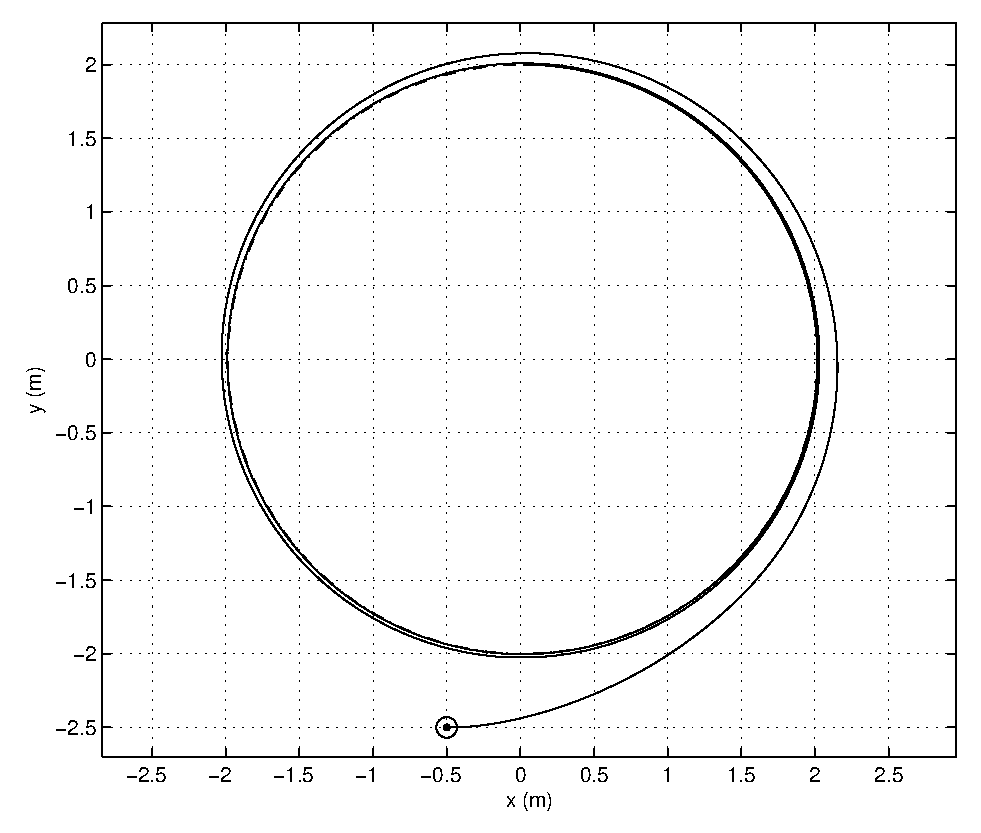
\includegraphics[width=\linewidth]{Figuras/traj_01.eps}
    	\caption{Trajectory in the $XY$ plane.}
    	\label{fig:traj_01}
\end{figure}
\begin{figure}[htbp]
	\centering
    	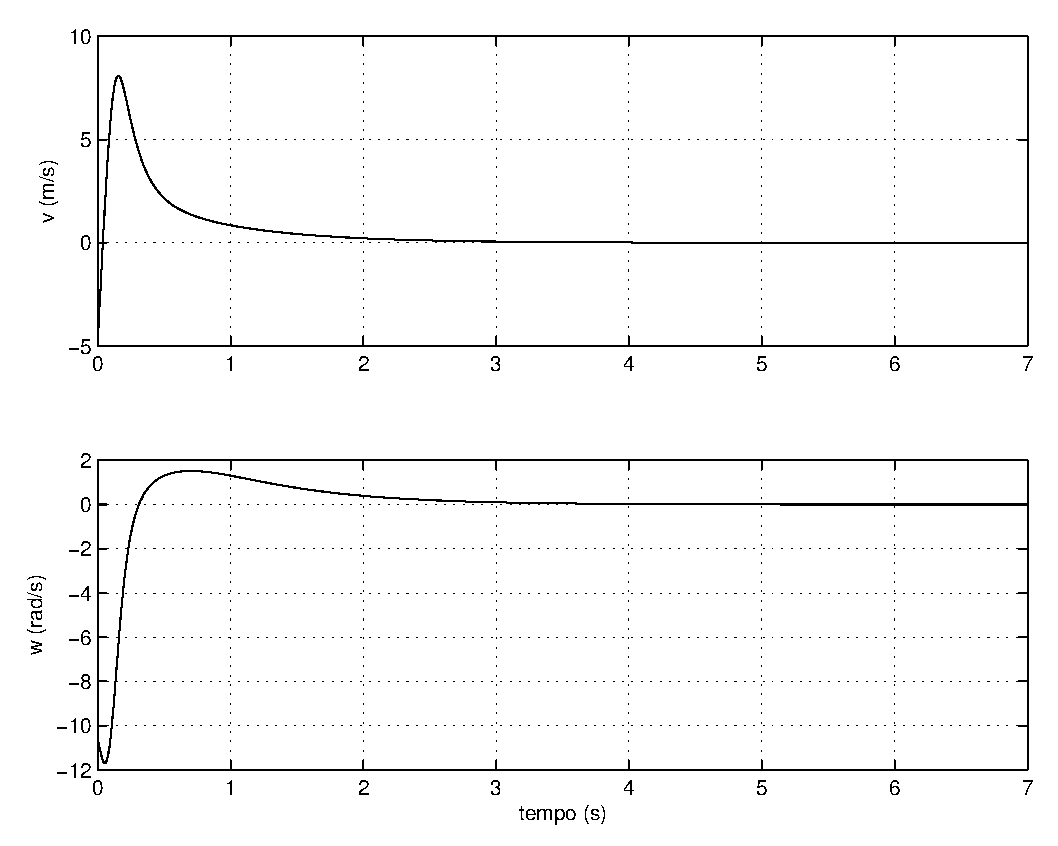
\includegraphics[width=\linewidth]{Figuras/control_01.eps}
    	\caption{Controls inputs.}
	\label{fig:control_01}
\end{figure}

It can be noted in Fig.~\ref{fig:traj_01} that the problem is successfully solved, but with low convergence rate. Fig.~\ref{fig:control_01} shows that the generated control signals respect the imposed constraints. The dash-dotted lines stands for the reference trajectories.

In the attempt of increasing the convergence rate,~\cite{essen01} proposed a modified cost function in order to increase the state penalty over the horizon, thus forcing the states to converge faster. Hence, the idea of exponentially increasing state weighting has been introduced. Also, a terminal state cost has been added to the cost function to be minimized. From these modifications the cost function assumes therefore the following form:
\begin{multline}\label{eqn:essencost}
	\Phi(k) = \sum_{j=1}^{N-1}\tilde{\bf x}^T(k+j|k){\bf Q}(j)\tilde{\bf x}(k+j|k) + \\ + \sum_{j=0}^{N-1}\tilde{\bf u}^T(k+j|k){\bf R}\tilde{\bf u}(k+j|k) + \Omega(\tilde{\bf x}(k+N|k)),
\end{multline}
where ${\bf Q}(j) = 2^{j-1}{\bf Q}$ and $\Omega(\tilde{\bf x}(k+N|k)) = \tilde{\bf x}^T(k+N|k){\bf P}\tilde{\bf x}(k+N|k)$, with ${\bf P}\geq 0$, is the terminal state cost.

Thus, by using the same conditions of the first case with ${\bf P}=30{\bf Q}(N)$, we have the results shown in Figures~\ref{fig:traj_02} and \ref{fig:control_02}.
\begin{figure}[htbp]
	\centering
   	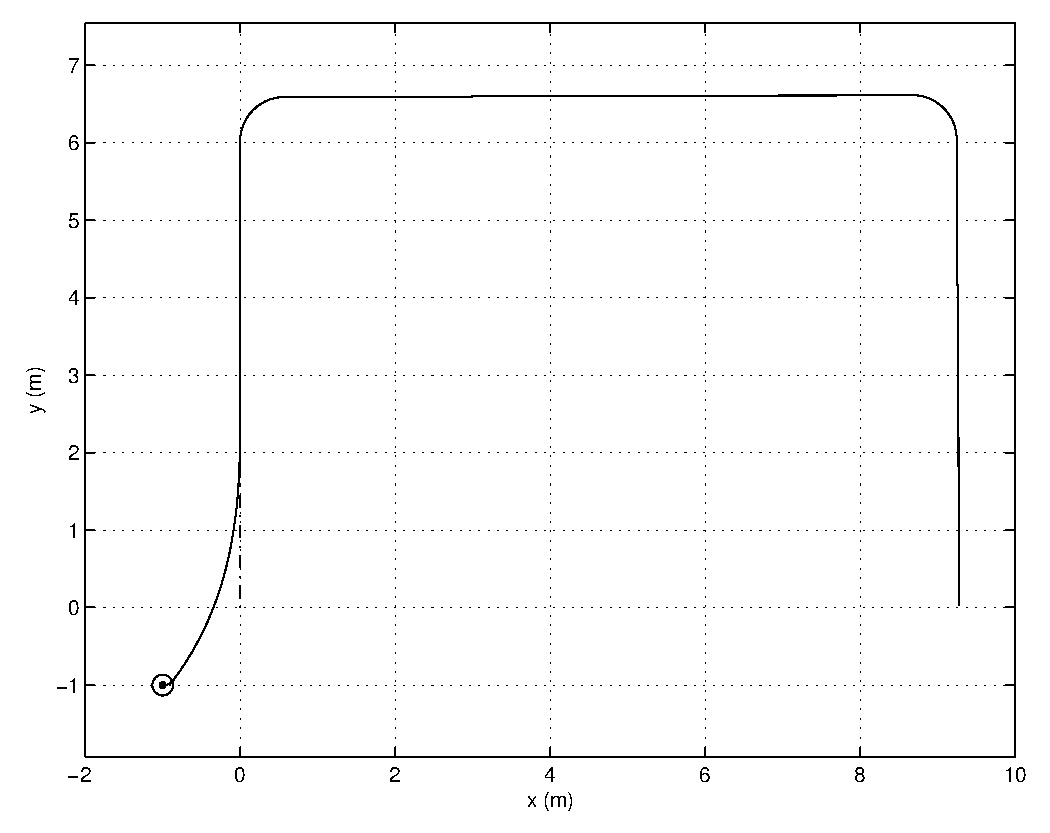
\includegraphics[width=\linewidth]{Figuras/traj_02.eps}
    	\caption{Trajectory in the $XY$ plane.}
    	\label{fig:traj_02}
\end{figure}
\begin{figure}[htbp]
	\centering
    	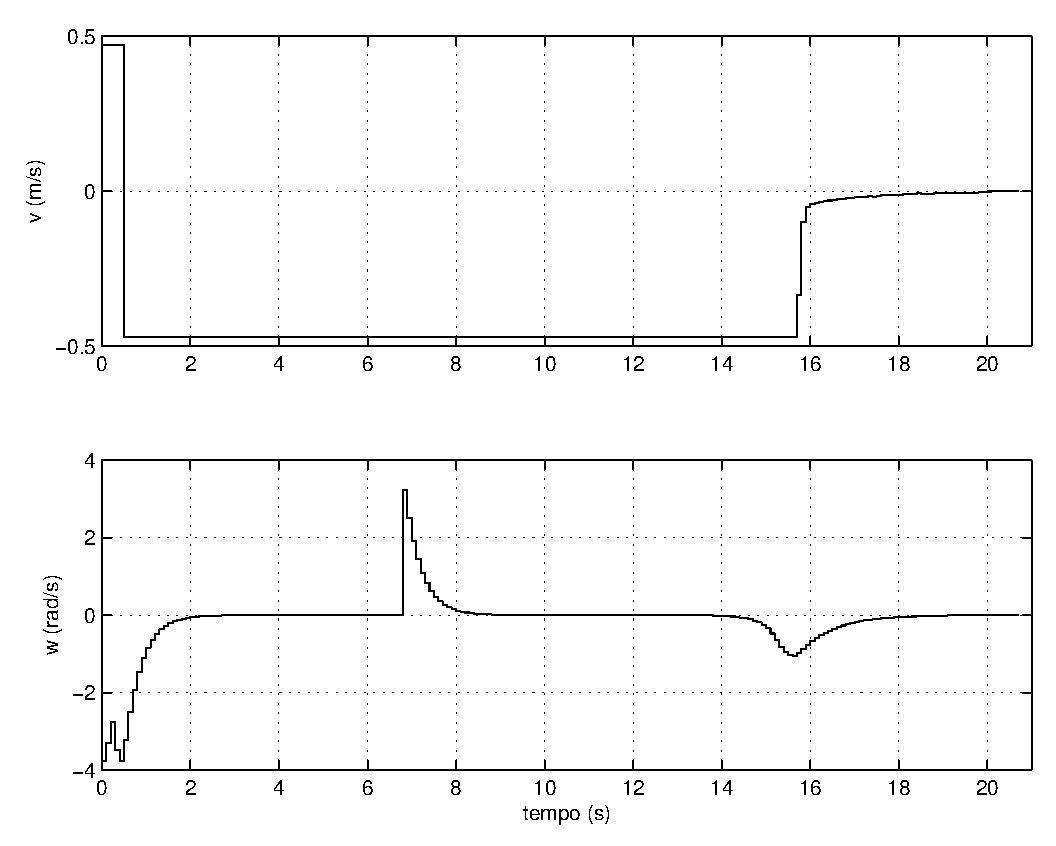
\includegraphics[width=\linewidth]{Figuras/control_02.eps}
    	\caption{Controls inputs.}
	\label{fig:control_02}
\end{figure}

Thus, comparing Fig.~\ref{fig:traj_01} and \ref{fig:traj_02}, it can be clearly seen that the robot presents a higher convergence rate, and Fig.~\ref{fig:control_02} shows that the control signals respect the imposed constraints.


%%%%%%%%%%%%%%%%%%%%%%%%%%%%%%%%%%%%%%%%%%%%%%%%%
\section{The Linear MPC Approach}\label{sec:lmpc}
In this section we introduce a linear MPC (LMPC) scheme applied to the problem of trajectory tracking.

Although many NMPC techniques has been proposed in the literature~\cite{chen98,allgower99}, it should be noticed that the computational effort necessary in this case is much higher than in the linear version. In NMPC there is a nonlinear programming problem to be solved on-line, which is nonconvex, has a larger number of decision variables and a global minimum is in general impossible to find~\cite{henson98}. In this section, we propose a strategy in order to reduce the computational burden. The fundamental idea consists in using a successive linearization approach, yielding a linear, time-varying description of the system. Then, considering the control inputs as the decision variables, it is possible to transform the optimization problem to be solved at each sampling time in a QP problem~\cite{kuhne05}. Since they are convex, QP problems can be easily solved by numerically robust algorithms which lead to global optimal solutions.

A linear model of the system dynamics can be obtained by computing an error model with respect to a reference car. By expanding the right side of \req{eqn:modelshort} in Taylor series around the point $({\bf x}_r,{\bf u}_r)$ and discarding the high order terms it follows that:
\begin{align*}\label{eqn:taylor2}
\dot{\bf x} = f({\bf x}_r,{\bf u}_r) &+ \left.\frac{\partial f({\bf x},{\bf u})}{\partial{\bf x}}\right|_{\begin{smallmatrix}{\bf x}={\bf x}_r \\
{\bf u}={\bf u}_r \end{smallmatrix}}({\bf x}-{\bf x}_r) + \\
&+ \left.\frac{\partial f({\bf x},{\bf u})}{\partial{\bf u}}\right|_{\begin{smallmatrix}{\bf x}={\bf x}_r \\
{\bf u}={\bf u}_r \end{smallmatrix}}({\bf u}-{\bf u}_r),
\end{align*}
or,
\begin{equation}\label{eqn:taylor}
	\dot{\bf x} = f({\bf x}_r,{\bf u}_r) + f_{{\bf x},r}({\bf x}-{\bf x}_r) + f_{{\bf u},r}({\bf u}-{\bf u}_r),
\end{equation}
where $f_{{\bf x},r}$ and $f_{{\bf u},r}$ are the jacobians of $f$ with respect to ${\bf x}$ and ${\bf u}$, respectively, evaluated around the reference point $({\bf x}_r,{\bf u}_r)$.
Then, the subtraction of~\req{eqn:refmodel} from~\req{eqn:taylor} results in:
\begin{equation*}\label{eqn:conterror}
	{\dot{\tilde{\bf x}}} = f_{{\bf x},r}\tilde{\bf x}+f_{{\bf u},r}\tilde{\bf u},
\end{equation*}
where, $\tilde{\bf x}={\bf x}-{\bf x}_r$ represents the error with respect to the reference car and $\tilde{\bf u}={\bf u}-{\bf u}_r$ is its associated error control input.

The approximation of $\dot{\bf x}$ by using forward differences gives the following discrete-time system model:

\begin{equation}
\label{eqn:error}
	\tilde{\bf x}(k+1) = {\bf A}(k)\tilde{\bf x}(k)+{\bf B}(k)\tilde{\bf u}(k),
\end{equation}
with
\begin{align*}
	{\bf A}(k) &= \begin{bmatrix}
		1 & 0 & -v_r(k)\sin\theta_r(k)T \\
		0 & 1 &  v_r(k)\cos\theta_r(k)T \\
		0 & 0 & 1
	\end{bmatrix} \\
	{\bf B}(k) &= \begin{bmatrix}
		\cos\theta_r(k)T & 0 \\
		\sin\theta_r(k)T & 0 \\
		0 			  & T
	\end{bmatrix}
\end{align*}

In~\cite{bloch89} it is shown that the nonlinear, nonholonomic system~\req{eqn:model} is fully controllable, i.e., it can be steered from any initial state to any final state by using finite inputs. On the other hand, it is easy to see that when the robot is not moving (i.e., $v_r=0$), the linearization around a stationary operating point is not controllable. However, this linearization becomes controllable as long as the control input ${\bf u}$ is not zero~\cite{samson91}. This implies that the tracking of a reference trajectory is possible with linear MPC.

Now it is possible to recast the optimization problem in an usual quadratic programming form. Hence, we introduce the following vectors:
\begin{equation*}
	\bar{\bf x}(k+1) = \begin{bmatrix}
		\tilde{\bf x}(k+1|k) \\ \tilde{\bf x}(k+2|k) \\ \vdots \\ \tilde{\bf x}(k+N|k) 
	\end{bmatrix},~
	\bar{\bf u}(k) = \begin{bmatrix}
		\tilde{\bf u}(k|k)  \\ \tilde{\bf u}(k+1|k) \\ \vdots \\ \tilde{\bf u}(k+N-1|k)
	\end{bmatrix}
\end{equation*}

Thus, with $\bar{\bf Q}={\rm diag}({\bf Q};\ldots;{\bf Q})$ and $\bar{\bf R}={\rm diag}({\bf R};\ldots;{\bf R})$, the cost function~\req{eqn:cost} can be rewritten as:
\begin{equation}\label{eqn:cost2}
	\Phi(k) = \bar{\bf x}^T(k+1)\bar{\bf Q}\bar{\bf x}(k+1) + \bar{\bf u}^T(k)\bar{\bf R}\bar{\bf u}(k),
\end{equation}

Therefore, it is possible from~\req{eqn:error} to write $\bar{\bf x}(k+1)$ as~\cite{kuhne05}:
\begin{equation}\label{eqn:exbar}
	\bar{\bf x}(k+1) = \bar{\bf A}(k)\tilde{\bf x}(k|k)+\bar{\bf B}(k)\bar{\bf u}(k),
\end{equation}
where $\bar{\bf A}$ and $\bar{\bf B}$ are defined in~\req{eqn:bigmtx} with $\alpha(k,j,l)$ given by:
\begin{equation*}
	\alpha(k,j,l) = \prod_{i=N-j}^{l}{\bf A}(k+i|k)
\end{equation*}
From~\req{eqn:cost2},~\req{eqn:exbar} and after some algebraic manipulations, we can rewrite the objective function~\req{eqn:cost} in a standard quadratic form:
\begin{equation}\label{eqn:cost3}
	\bar\Phi(k) = \frac{1}{2}\bar{\bf u}^T(k){\bf H}(k)\bar{\bf u}(k) + {\bf f}^T(k)\bar{\bf u}(k) + {\bf d}(k)
\end{equation}
with
\begin{align*}
	{\bf H}(k) &= 2\left(\bar{\bf B}(k)^T(k)\bar{\bf Q}\bar{\bf B}(k)+\bar{\bf R}\right) \\
	{\bf f}(k) &= 2\bar{\bf B}^T(k)\bar{\bf Q}\bar{\bf A}(k)\tilde{\bf x}(k|k) \\
	{\bf d}(k) &= \tilde{\bf x}^T(k|k)\bar{\bf A}^T(k)\bar{\bf Q}\bar{\bf A}(k)\tilde{\bf x}(k|k)
\end{align*}

\twocolumn[
\begin{equation}\label{eqn:bigmtx}
	\bar{\bf A}(k) = \begin{bmatrix}
		{\bf A}(k|k) \\ {\bf A}(k+1|k){\bf A}(k|k) \\ \vdots \\ \alpha(k,2,0) \\ \alpha(k,1,0)
	\end{bmatrix} \quad
	\bar{\bf B}(k) = \begin{bmatrix}
			{\bf B}(k|k)		       & {\bf 0} 			    	  & \cdots & {\bf 0}         \\
			{\bf A}(k+1|k){\bf B}(k|k) & {\bf B}(k+1|k)      	       & \cdots & {\bf 0}         \\
			\vdots			       & \vdots			  	  & \ddots & \vdots          \\
			\alpha(k,2,1){\bf B}(k|k)  & \alpha(k,2,2){\bf B}(k+1|k) & \cdots & {\bf 0}	    \\
			\alpha(k,1,1){\bf B}(k|k)  & \alpha(k,1,2){\bf B}(k+1|k) & \cdots & {\bf B}(k+N-1|k)
		\end{bmatrix}
\end{equation}

\rule{\linewidth}{.1pt}
\\

]

The matrix ${\bf H}(k)$ is a {\em Hessian} matrix, and it is always positive definite. It describes the quadratic part of the objective function, and the vector ${\bf f}$ describes the linear part. $\bf d$ is independent of $\tilde{\bf u}$ and has no influence in the determination of $\bf u^\star$. Thus, we define
\begin{equation*}
	\bar\Phi'(k) = \frac{1}{2}\bar{\bf u}^T(k){\bf H}(k)\bar{\bf u}(k) + {\bf f}^T(k)\bar{\bf u}(k),
\end{equation*}	
which is a standard expression used in QP problems and the optimization problem to be solved at each sampling time is stated as follows:
\begin{equation}\label{eqn:optim2}
	\tilde{\bf u}^\star = \arg\min_{\tilde{\bf u}}\left\{\bar\Phi'(k)\right\}
\end{equation}
s. a.
\begin{equation}\label{eqn:restu2}
	{\bf D\tilde u}(k+j|k) \leq {\bf d}, ~~j~\in[0,N-1]
\end{equation}

Note that now only the control variables are used as decision variables. Furthermore, constraints for the initial condition and model dynamics are not necessary anymore, since now these informations are implicit in the cost function~\req{eqn:cost3}, and any constraint must be written with respect to the decision variables (constraint~\req{eqn:restu2}). In this case, the amplitude constraints in the control variables of~\req{eqn:restu} can be rewritten as ${\bf u}_{min} - {\bf u}_r(k+j) \leq \tilde{\bf u}(k+j|k) \leq {\bf u}_{max} - {\bf u}_r(k+j)$, and we have that:
\begin{equation*}
	{\bf D} = \begin{bmatrix} {\bf I} \\ -{\bf I} \end{bmatrix}, \qquad 
	{\bf d} = \begin{bmatrix} {\bf u}_{max}-{\bf u}_r(k+j) \\ {\bf u}_{min}+{\bf u}_r(k+j) \end{bmatrix}
\end{equation*}

Since the state prediction is a function of the optimal sequence to be computed, it is easy to show that state constraints can also be cast in the generic form given by~\req{eqn:restu2}. Furthermore, constraints on the control rate and states can also be formulated in a similar way.

Using the same procedure above, the matrix ${\bf H}(k)$ and the vectors ${\bf f}(k)$ and ${\bf d}(k)$ can be easily rewritten in order to consider the more generic cost function~\req{eqn:essencost}. In this case it suffices to consider $\bar{\bf Q}$ in~\req{eqn:cost3} as $\bar{\bf Q}={\rm diag}(2^0{\bf Q},2^1{\bf Q},\ldots,2^{N-1}{\bf P})$, where $\bf P$ is the terminal state penalty matrix. Considering the same data used in the cases previously shown, the optimization problem~\req{eqn:optim2}--\req{eqn:restu2} is solved at each sampling time. Figures~\ref{fig:traj_03}--\ref{fig:control_03} show the simulation results\footnote{The optimization problem was solved with the {\sc Matlab} routine {\tt quadprog}.} in this case, where the dash-dotted lines stand for the reference trajectories and the dashed line stand for the trajectories of the nonlinear case (Figures~\ref{fig:traj_02} and \ref{fig:control_02}).
\begin{figure}[t]
	\centering
   	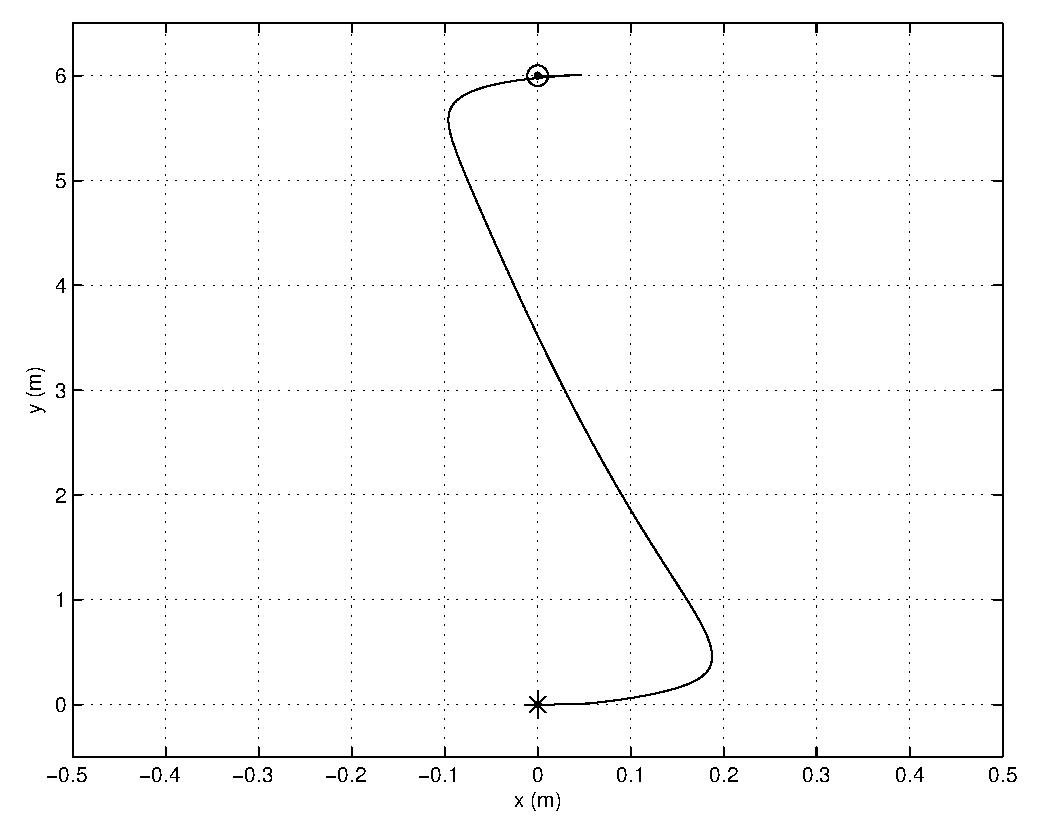
\includegraphics[width=\linewidth]{Figuras/traj_03.eps}
    	\caption{Trajectory in the $XY$ plane.}
    	\label{fig:traj_03}
\end{figure}
\begin{figure}[H]
	\centering
    	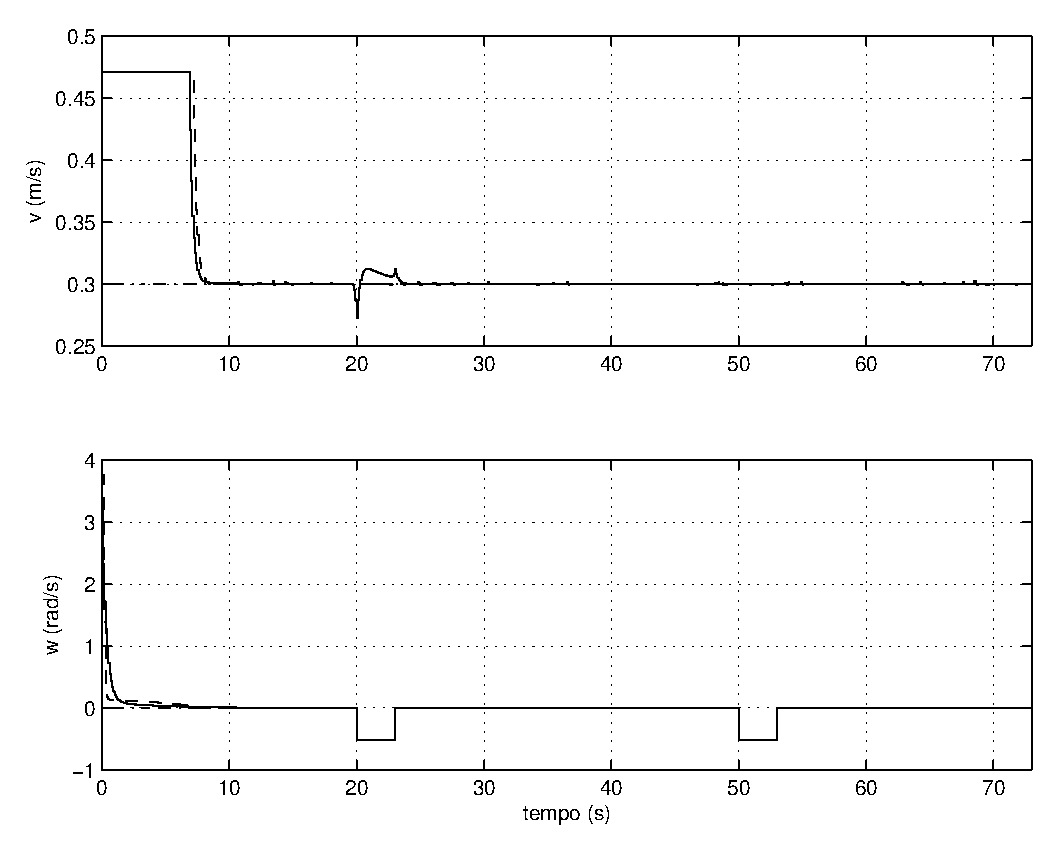
\includegraphics[width=\linewidth]{Figuras/control_03.eps}
    	\caption{Controls inputs.}
	\label{fig:control_03}
\end{figure}

It can be seen that there are not significative difference between the nonlinear (Figures~\ref{fig:traj_02} and \ref{fig:control_02}) and linear cases (Figures~\ref{fig:traj_03} and \ref{fig:control_03}). Once more, the computed control signals respect the imposed constraints.

%%%%%%%%%%%%%%%%%%%%%%%%%%%%%%
\section{Computational Effort}
The use of MPC for real-time control of systems with fast dynamics such as a WMR has been hindered for some time due to its numerical intensive nature~\cite{cannon00}. However, with the development of increasingly faster processors the use of MPC in demanding applications becomes possible. 

In order to evaluate the real-time implementability of the proposed MPC, we consider, as measurement criterion, the number of floating point operations per second (flops). With this aim we consider that the computations run in an Athlon XP 2600+ which is able to perform a peak performance between 576 and 1100 Mflops accordingly to~\cite{aburto92}, a de-facto standard for floating point performance measurement.

The sampling period used in all examples presented here is $T=100~ms$. The data in Table~\ref{tab:comp} refers to the mean values of Mflops along the developed trajectory, for a MPC applied to the trajectory tracking with cost function of~\cite{essen01}. 

\begin{table}[H]
	\renewcommand{\arraystretch}{1.2}
	\caption{Computational Effort.}
	\centering
 	\begin{tabular}{c|cc}
  		\hline
  				& \multicolumn{2}{c}{Mflops} \\
          Horizon 	& NMPC & LMPC \\
  		\hline\hline
  		5	& 11.1 & 0.17 \\
  		10	& 502 & 0.95 \\
  		15	& 5364 & 3.5 \\
  		20	& --- & 9.1  \\
  		\hline
 	\end{tabular}
	\label{tab:comp} 	
\end{table}

The data in Table~\ref{tab:comp} provides enough evidence that a standard of-the-shelf computer is able to run a MPC-based controller for a WMR. Note that for $N=5$ both cases are feasible in real-time. It is important to note the difference between the nonlinear and linear cases. For a horizon higher than 10, the NMCP would not be applicable, while the LMPC presents admissible computational effort for a horizon of 20 or even higher. On the other hand, comparing the performance showed in Fig.~\ref{fig:traj_03} and Table~\ref{tab:comp}, we can say that the linear approach developed here is a good alternative when lower computational effort is necessary since it does not presents a significative loss n performance.

%%%%%%%%%%%%%%%%%%%%%%%%%%%%%%%%%%%%%%%%%%%
\section{Conclusion}\label{sec:conclusions}

This paper has presented an application of MPC to solve the problem of mobile robot trajectory tracking. Two approaches have been presented, first with nonlinear MPC (leading to a non-convex optimization problem) and after that with linear MPC (by recasting the problem as a quadratic programming one). The obtained control signals are such that the constraints imposed on the control variables are respected and the convergence rates are improved by some modifications in the cost function. 

In addition, a study regarding the computational effort necessary to solve the optimization problems has been carried out in order to evaluate the implementability of the proposed schemes in real-time.

With the linear approach, it has been possible to reduce the computational effort, since the MPC optimization problem has been recasted as a QP one. In comparison with the nonlinear approach, it has been noted that the linear strategy maintains good performance, with lower computational effort. It is important to point out that the LMPC has the disadvantage that the linearized model is only valid for points near the reference trajectory. However, this problem can be easily solved with the {\em pure-pursuit} strategy~\cite{rico99}.

%The choice of MPC for the application given here is well justified by some advantages: the straightforward way in which state/input constraints can be handled; the existence of a performance criterion to be minimized; the tuning parameters are directly related to the performance index.

%%%%%%%%%%%%%%%%%%%%%%%%%%
\section*{Acknowledgments}
The authors gratefully acknowledge the financial support from CAPES and CNPq, Brazil.

%\bibliographystyle{dcu}
\bibliography{sbai05}

\end{document}
